\documentclass[journal,12pt,onecolumn,draftclsnofoot]{IEEEtran}
\usepackage{blindtext}
\usepackage{graphicx}
\usepackage[T1]{fontenc}
\usepackage{tabulary}
\usepackage{booktabs}
\usepackage{cite}
\usepackage[cmex10]{amsmath}
\usepackage{hyperref}
\usepackage[mathscr]{euscript}
\usepackage{algorithm}
\usepackage{algorithmic}
\usepackage{listings}
\usepackage{color}
\usepackage[table]{xcolor}
\usepackage{caption} % Load the caption package
\usepackage{float}

% Ensure captions are centered
\captionsetup{
    justification=centering
}
% Define colors for MATLAB listing
\definecolor{mygreen}{rgb}{0,0.6,0}
\definecolor{mygray}{rgb}{0.5,0.5,0.5}
\definecolor{mymauve}{rgb}{0.58,0,0.82}
\definecolor{mylilas}{RGB}{170,55,241}

% Setup the language (MATLAB), including color and style of syntax highlighting
\lstset{language=Matlab,
    basicstyle=\footnotesize\ttfamily,
    breaklines=true,
    morekeywords={matlab2tikz},
    keywordstyle=\color{blue},
    morekeywords=[2]{1}, keywordstyle=[2]{\color{black}},
    identifierstyle=\color{black},
    commentstyle=\color{mygreen},
    stringstyle=\color{mymauve},
    showstringspaces=false,
    numbers=left,
    numberstyle=\tiny\color{mygray},
    numbersep=9pt,
    emph=[1]{for,end,break},emphstyle=[1]\color{red},
}

\usepackage{amssymb}
\usepackage{tikz}

\begin{document}

\title{Nonnegative matrix factorization with gradient descent}

\author{Mohammad~Mashreghi - 810199492}

\maketitle

\begin{abstract}
This project explores the application of Nonnegative Matrix Factorization (NMF) using Gradient Descent Algorithm (GDA) for face recognition on the CBCL FACE database. The primary goal is to decompose a given nonnegative matrix \( V \) into the product of two nonnegative matrices \( W \) and \( H \), minimizing the Frobenius norm of their difference. Our approach involved implementing the GDA as per Lee \& Seung (2001), where the matrices \( W \) and \( H \) are updated iteratively while ensuring their nonnegativity. The algorithm was tested on normalized face data with a dimension reduction parameter \( k = 49 \), running over 300 iterations. Results include a visualization of the basis images represented by the columns of \( W \) and a plot of the objective function over iterations, reflecting the convergence of the method. The project demonstrates the effectiveness of GDA in maintaining nonnegative constraints during matrix updates, crucial for the feasibility of solutions in practical applications such as image reconstruction. Reconstructed faces showed a promising fidelity to original test images, as quantified by the mean squared error of reconstructions. This study not only reinforces the utility of NMF in image processing but also illustrates the potential of gradient-based optimization methods in handling large-scale data with inherent nonnegativity.
\end{abstract}

\section*{A : Normalization of Face Images}

The function \texttt{normalize\_faces} is used to preprocess face images for Nonnegative Matrix Factorization. This MATLAB function normalizes the images by adjusting their median and scaling their deviations to enhance the robustness of the NMF algorithm. Below is the MATLAB code used:

\begin{lstlisting}
function V_normalized = normalize_faces(V)
    V = dlmread('face.txt', ' ');
    
    V_normalized = zeros(size(V));
    
    for i = 1:size(V, 2)
        face = V(:, i);
        
        median_face = median(face);
        face = face - median_face + 0.5;
        
        median_deviation = median(abs(face - 0.5));
        face = 0.5 + (face - 0.5) * (0.25 / median_deviation);
        
        face(face < 1e-4) = 1e-4;
        face(face > 1) = 1;
        
        V_normalized(:, i) = face;
    end
    
    dlmwrite('face_normalized.txt', V_normalized, ' ');
end
\end{lstlisting}
\par

Resulting Image of Normalized Faces:

\begin{figure}[h]
    \centering
    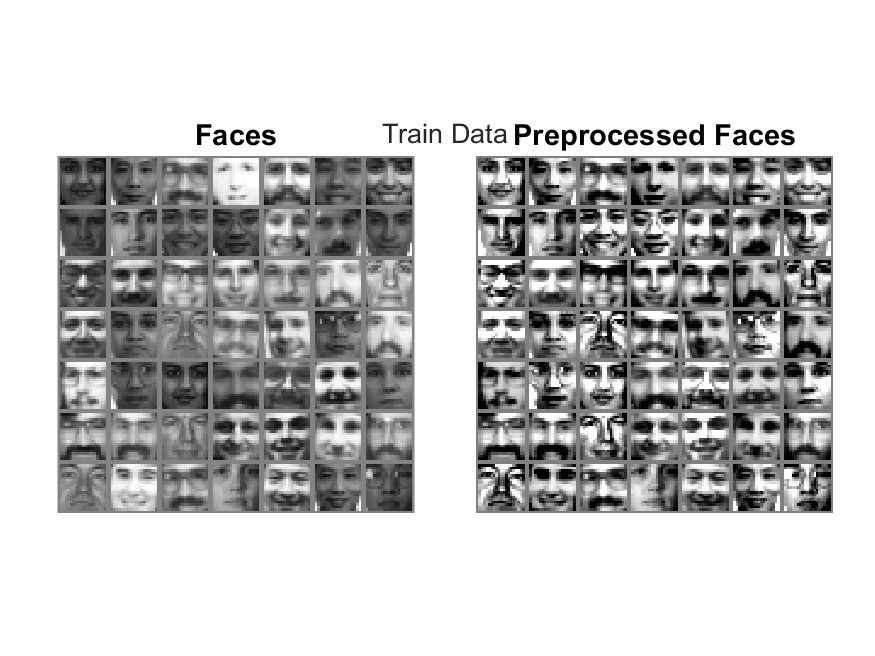
\includegraphics[width=0.8\textwidth]{images/TrainData.jpeg}
    \caption{Normalized faces from the training dataset.}
    \label{fig:normalized_faces}
\end{figure}




\section*{B : Matrix Factorization and Optimization}

In this section, we implement the Nonnegative Matrix Factorization (NMF) using gradient descent optimization. The update rules for the matrices $H$ and $W$ are derived to minimize the Frobenius norm of the difference between the original matrix $V$ and the product $WH$. 

These update rules are given by:

\[
H \leftarrow H \frac{(W^TV)}{(W^TWH) }
\]

\[
W \leftarrow W \frac{(VH^T)}{(WHH^T) }
\]


The MATLAB function \texttt{nmf} is implemented as follows to perform the matrix updates and calculate the objective values over iterations, which measure the convergence of the algorithm:

\begin{lstlisting}
function [W, H, obj_vals] = nmf(V, k, max_iter)
    [m, n] = size(V); % Dimensions of the input matrix
    
    W = rand(m, k); % Initialize W randomly
    H = rand(k, n); % Initialize H randomly
    
    obj_vals = zeros(max_iter, 1); % Initialize the array to store objective values
    
    for iter = 1:max_iter
        % Update H using element-wise multiplication and division
        H = H .* ((W' * V) ./ (W' * W * H ));
        
        % Update W using element-wise multiplication and division
        W = W .* ((V * H') ./ (W * H * H' ));
        
        % Compute the Frobenius norm of the difference between V and WH
        obj_vals(iter) = norm(V - W * H, 'fro')^2;
    end
end
\end{lstlisting}

These iterative updates progressively reduce the discrepancy between $V$ and $WH$, as evidenced by the objective values calculated at each iteration.



\subsubsection*{Convergence of NMF}
In this part, after 300 iter the  objective value reach about 10000 which it change when we select 49 random picture each time.
\begin{figure}[htbp]
    \centering
    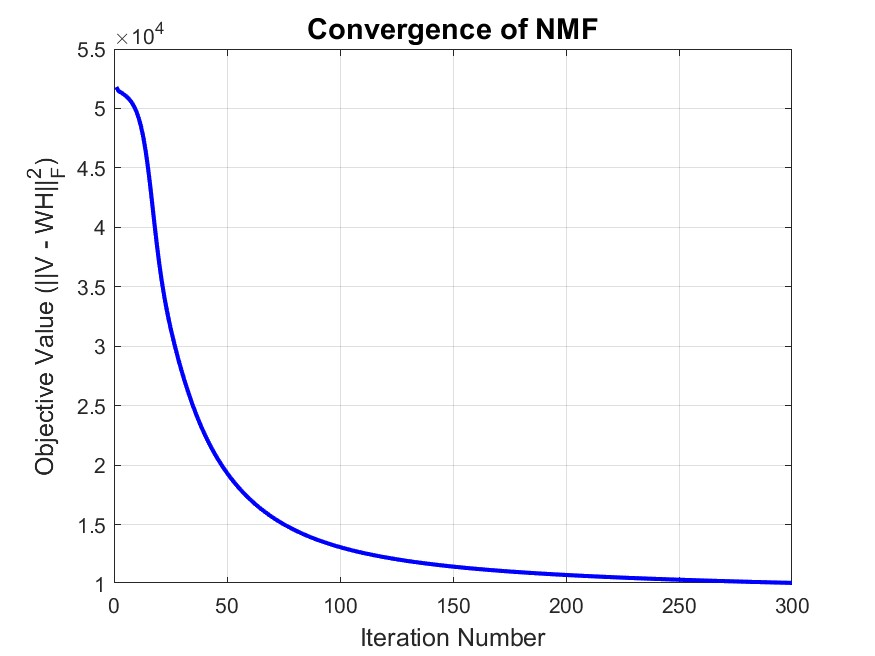
\includegraphics[width=0.8\textwidth]{images/NMF_Convergence.jpeg}
    \caption{Convergence of the NMF algorithm showing the decrease in objective value over iterations.}
    \label{fig:nmf_convergence}
\end{figure}

\subsubsection*{Learned Basis Elements (gray \& inverse gray)}
\mbox{}\\
\begin{figure}[H]
    \centering
    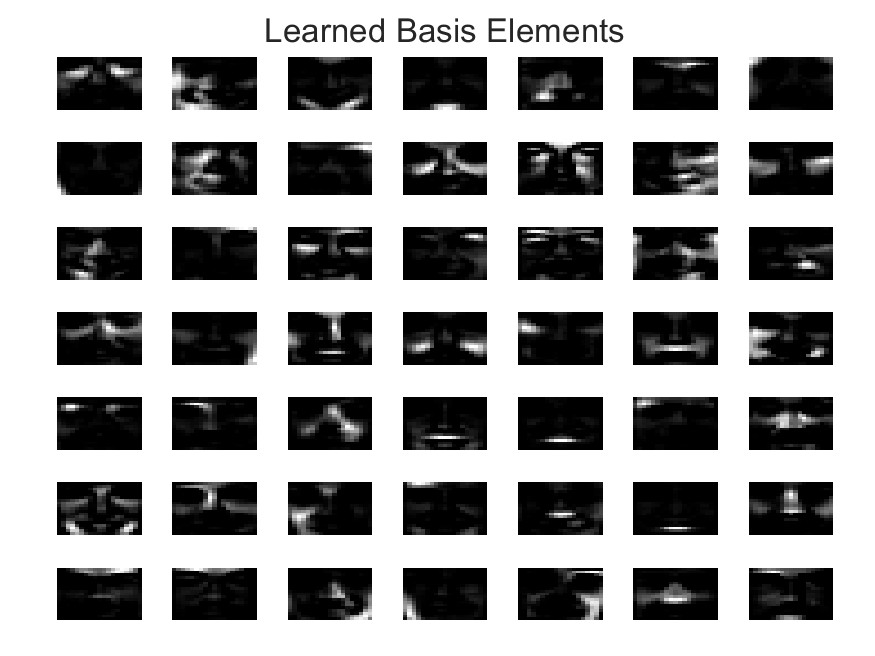
\includegraphics[width=0.8\textwidth]{images/Learned_BasisElements.jpeg}
    \caption{Visual representation of the basis elements learned through NMF.}
    \label{fig:learned_basis_elements}
\end{figure}

\begin{figure}[H]
    \centering
    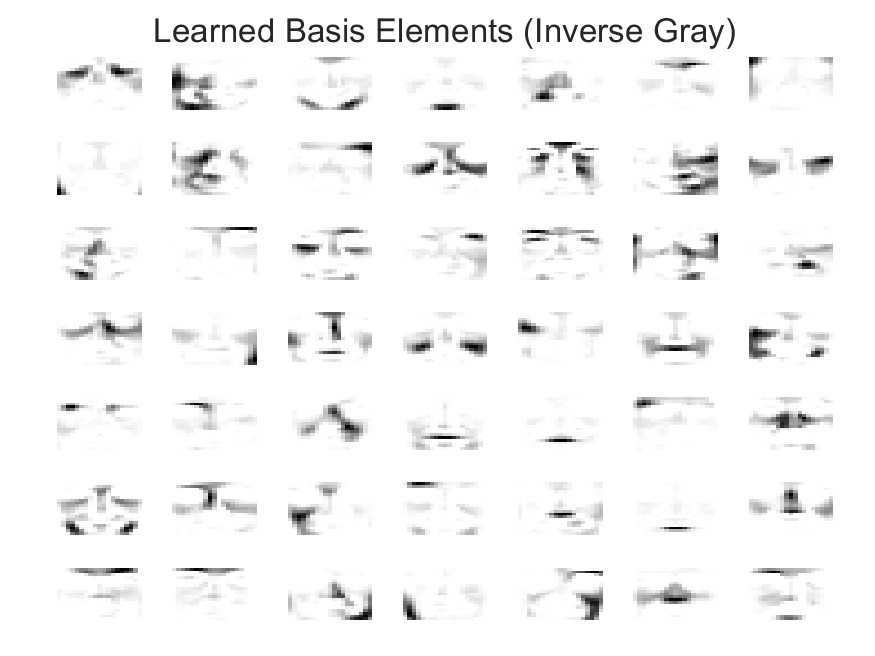
\includegraphics[width=0.8\textwidth]{images/Learned_BasisElements_Inverse.jpeg}
    \caption{Learned basis elements displayed with an inverse grayscale colormap.}
    \label{fig:learned_basis_elements_inverse}
\end{figure}
As can be seen from both images, It can be understood that it tries to learn the shape of faces. For example in inverse Gray image

\section*{C : Algorithm Interpretation and Gradient Descent}

\subsection*{Gradient Descent Update Rules}
The algorithm can be understood in this way, considering the objective function:
\[
J = \|V - WH\|^2_F
\]
If \(W\) is held constant:
\[
\frac{1}{2} (\nabla_H J)_{ij} = (W^T)_{ji} (V - WH)_{ij}
\]
Updating \(H\):
\[
H_{ij} = H_{ij} + \alpha_{ij} (\nabla_H J)_{ij}
\]
If \(\alpha_{ij} = 2 \frac{H_{ij}}{(W^T WH)_{ij}}\):
\[
H_{ij} = H_{ij} + \frac{H_{ij} (W^T)_{ji} (V - WH)_{ij}}{(W^T WH)_{ij}} = H_{ij} \left( 1 + \frac{(W^T V)_{ij} - (W^T WH)_{ij}}{(W^T WH)_{ij}} \right) = H_{ij} \frac{(W^T V)_{ij}}{(W^T WH)_{ij}}
\]

Also we can say for \(W\):
\[
W_{ij} = W_{ij} \frac{(VH^T)_{ij}}{(WHH^T)_{ij}}
\]

\subsection*{Alternative Objective Function}
Since the matrices \(V\), \(W\), and \(H\) are composed entirely of non-negative elements, the updates designed for \(W\) and \(H\) within the gradient descent framework inherently preserve this non-negativity. This is critical because non-negative matrices are often used to represent data with inherent positivity, such as image data and probability distributions, where negative values would be non-physical or invalid.
To enhance the algorithm's applicability and performance, an alternative method modifies the objective function by minimizing a divergence measure instead of using the Frobenius norm \( \|V - WH\|_F^2 \). This approach, which is particularly suitable for probabilistic data, adjusts the update rules in Non-negative Matrix Factorization (NMF) to minimize the divergence between the actual data \( V \) and its approximation \( WH \). This allows for a more effective alignment of distributions compared to simply minimizing their numerical differences. (from the paper:)
\[
D(A||B) = \sum_{ij} \left( A_{ij} \log \frac{A_{ij}}{B_{ij}} - A_{ij} + B_{ij} \right)
\]
The update rule is as follows:
\[
H_{ap} \leftarrow H_{ap} \frac{\sum_i W_{ia} V_{ip} / (WH)_{ip}}{\sum_k W_{ka}}
\]
this also be analyzed as a gradient descent method:
\[
H_{ap} \leftarrow H_{ap} + \eta_{ap} \left( \sum_i W_{ia} \frac{V_{ip}}{(WH)_{ip}} - \sum_i W_{ia} \right)
\]
which \[\eta_{ap}\] is:
\[
\eta_{ap} = \frac{H_{ap}}{\sum_i W_{ia}}
\]


\section*{D : Test Faces}



In our experiment, we load the test face images (contained in \texttt{face test.txt}) and reconstruct them using a fixed, pre-learned basis matrix $W$. We optimize the coefficient matrix $H \in \mathbb{R}^{k \times n_{\text{test}}}$ using multiplicative updates, while keeping $W$ fixed. At each iteration, the reconstruction error is computed as:
\begin{equation}
    J = \|V_{\text{test}} - W H\|_F^2,
\end{equation}
where $V_{\text{test}} \in \mathbb{R}^{m \times n_{\text{test}}}$ is the matrix of normalized test face images. After 300 iterations, the mean-squared-error per image is given by:
\begin{equation}
    \text{MSE per image} = \frac{J}{n_{\text{test}}}.
\end{equation}
Figure~\ref{fig:reconstruction} shows the reconstructed faces compared to the original test faces (see the image \texttt{TestData\_Reconstruction.jpeg} in the images folder).

Below is the MATLAB function used for testing:

\begin{lstlisting}
function [objective_val_history, H] = test_faces(W, testV_normalized)
    max_iter = 300;
    
    [m, n_test] = size(testV_normalized);
    k = size(W, 2);
    
    H = rand(k, n_test);
    
    objective_val_history = zeros(max_iter, 1);
    
    for iter = 1:max_iter
        H = H .* ((W' * testV_normalized) ./ (W' * W * H ));
        objective_val_history(iter) = norm(testV_normalized - W * H, 'fro')^2;
    end
end
\end{lstlisting}

\begin{figure}[ht]
    \centering
    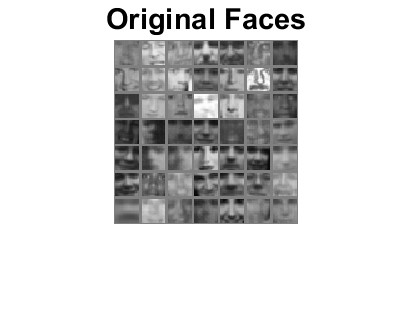
\includegraphics[width=0.8\linewidth]{images/OriginalFaces_partD.jpeg}
    \caption{Original test faces.}
    \label{fig:OriginalFaces}
\end{figure}
\begin{figure}[ht]
    \centering
    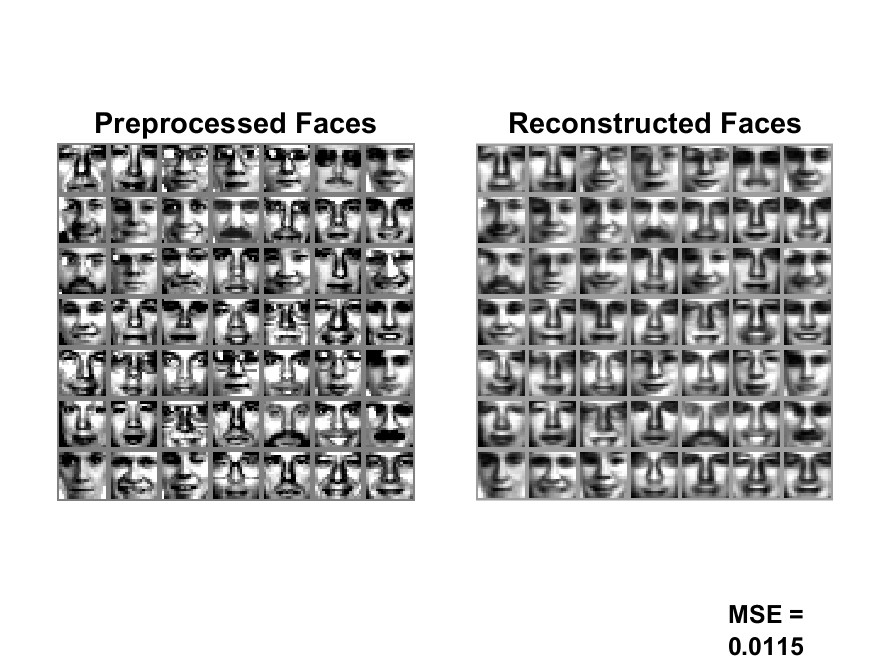
\includegraphics[width=0.8\linewidth]{images/Preprocessed_Reconstructed.jpeg}
    \caption{Reconstructed faces versus the Preprocessed test faces.}
    \label{fig:reconstruction}
\end{figure}

\begin{figure}[ht]
    \centering
    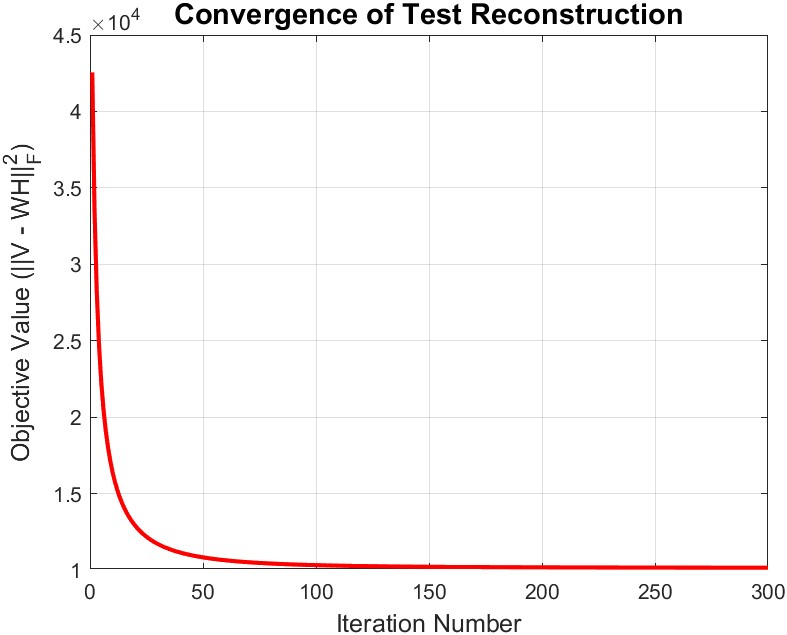
\includegraphics[width=0.8\linewidth]{images/untitled2.jpg}
    \caption{Converge of the test reconstruction}
    \label{fig:reconstruction}
\end{figure}


As can be seen, Reconstructed faces are similar to the preprocessed faces. And the MSE is 0.0115 which for each image is about 0.000237 which shows that these two cluster look the same. which the last figure makes it clear.

\end{document}
